%!TEX program = xelatex
\documentclass[10pt, compress]{beamer}
\usetheme{Marburg}
\usepackage{tikz}
\setbeamertemplate{caption}{\raggedright\insertcaption\par}
\usetheme{m}
\usepackage{color}
\usepackage{booktabs}
\usepackage[scale=2]{ccicons}
%\usepackage{minted}
\usepackage{media9}

\usepgfplotslibrary{dateplot}

%\usemintedstyle{trac}

\title[The potential of 3D printing in modern Chemistry]{The potential of 3D printing in modern Chemistry
	\hspace{4cm} \includemedia[
	label=testsound,
	addresource=test.mp3,
	activate=pageopen,
	flashvars={source=test.mp3&autoPlay=true&hideBar=true},
	transparent
	]{\fbox{\small{Click for voiceover}}}{APlayer.swf}}
\date{\today}
\author{Alexander Papiez}
\institute{Northumbria University}

\begin{document}

\maketitle

\begin{frame}[fragile]
  \frametitle{Overview
			  \hspace{3cm}\includemedia[
		  	    label=testsound,
		  	    addresource=test.mp3,
		  	    activate=pageopen,
		  	    flashvars={source=test.mp3&autoPlay=true&hideBar=true},
		  	    transparent
		  	    ]{\fbox{\small{Click for voiceover}}}{APlayer.swf}
}
  \vspace{-1cm}
	\tableofcontents
  
\end{frame}

\section{Introduction}

\begin{frame}[fragile]
  \frametitle{The popular view of a chemistry lab...}
  \centering\includegraphics[scale=0.18]{Typical_Lab_glassware.png}
  
\end{frame}


%\begin{frame}[fragile]
	%\frametitle{A brief history of glassware}
    %\begin{tikzpicture}[thick,scale=0.8, every node/.style={scale=0.8}]
    %%%%%%%%%%%%%%% Draw the initial line for the timeline%%%%%%%%%
    %\coordinate (Point1) at (0, 0);
    %\coordinate (Point2) at (10, 0);
    %\draw[thick, color=black] (Point1) -- (Point2);
    %%%%%%%%%%%%%%%%%%%%%%%%%%%%%%%%%%%%%%%%%%%%%%%%%%%%%%%%%%%%%%%%
    %\draw[fill=black] (Point1) circle (0.1); %Black %circle at point 1
    %\node[rotate=45] (phonecians) at (0, -1) {\small{5000 B.C.}}; %rotated text
    %\draw (phonecians) -- (Point1); %line from point one to rotated text
    %\draw[thin] (Point1) -- (0, 0.5);
    %\node[rotate=45] (A) at (0, 1) {\tiny{Early Phonecians made use}};
    %\node[rotate=45] (Aa) at (0, 0.8) {\tiny{of glass beads for decorative purposes}};
    %\node[rotate=45] (B) at (5, 1) {\tiny{Glass vessels made}};
    %\node[rotate=45] (Bb) at (5, 0.8) {\tiny{By the anicent Egyptians}};
    %\draw[fill=black] (5, 0) circle (0.1);
    %\draw[thin] (5, 0) -- (5, 0.5);
    %\node[rotate=45] (1500bc) at (5, -1) {\small{1500 B.C.}};
    %\node[rotate=45] (100bc) at (7, -1) {\small{100 B.C.}};
    %\draw (7, 0) -- (7, -0.8);
    %\draw[fill=black] (7, 0) circle (0.1);
    %\node[rotate=45] (C) at (7, 1) {\tiny{Advent of}};
    %\node[rotate=45] (Ca) at (7, 0.8) {\tiny{glassblowing}};
    %\draw[thin] (7, 0) -- (7, 0.5);
    %\node[rotate=45] (buchner) at (7.96, 0.7) {\tiny{Development of the}};
    %\node[rotate=45] (buchner2) at (7.96, 0.5) {\tiny{Buchner Flask}};
    %\node[rotate=45] (18C) at (8, -1) {\small{1890}};
    %\node[rotate=45] (BSG) at (8, 2.5) {\tiny{Development of Borosilicate}};
    %\node[rotate=45] (BSG2) at (8, 2.3) {\tiny{glass by Otto Schott}};
    %\draw[thin] (8,1) -- (8, 2);
    %\draw[fill=black] (8, 0) circle (0.1);
    %\node[rotate=45] (Today) at (10, -1) {\small{2016}};
    %\draw (Today) -- (Point2);
    %\node[rotate=45] (tod1) at (10, 0.85) {\tiny{Development of microfluidics}};
    %\draw[fill=black] (Point2) circle (0.1);
    %\end{tikzpicture}
%\end{frame}

\begin{frame}[fragile]
\begin{itemize}
	\item{ Most of our current glassware was developed in the 19$^{th}$ century and has seen little change}
    \item{Why?}
    \item{Glass can be blown into any desired shape}
    \item{The advent of borosilicate glass means temperature is no longer a problem}
    \item{Transparent reaction vessels allow easy monitoring of reactions}
    \item{\color{red}However glassware production is centralized and few labs have direct access to a glassblower - increasing the difficulty of designing and obtaining bespoke glassware} 
\end{itemize}
\end{frame}

\section{Additive manufacturing: A 24$^{th}$ century technology?}
\begin{frame}[fragile]
\frametitle{Star Trek: Harbinger of the future}\vspace{-1cm}
\begin{center}\includegraphics[scale=0.43]{enterprise.png}\end{center}

\end{frame}

\begin{frame}[fragile]
\begin{center}\includegraphics[scale=0.75]{Coffee_replicates_then_mug.jpg}\end{center}
\end{frame}

\subsection{21st Century Replicators}
\begin{frame}[fragile]
\frametitle{21st Century replicators}
\begin{center}\includegraphics[width=.9\textwidth]{fig1.png}\end{center}
\end{frame}






\subsection{Why 3D Printing}
\subsubsection{Iterative Development}
\begin{frame}[fragile]
\frametitle{Why 3D printing?}
\begin{center}\includegraphics[width=.9\textwidth]{iterative_cycle.PNG}\end{center}


\end{frame}

\begin{frame}[fragile]
\subsubsection{Advancing the field to promote innovation}
\begin{center}
\begin{figure}[h !]
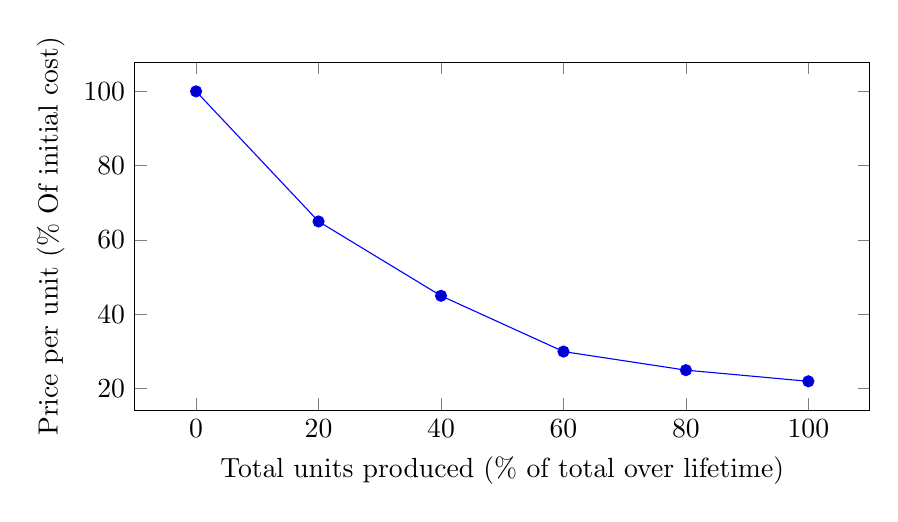
\begin{tikzpicture}
      \begin{axis}[
        xlabel={Total units produced (\% of total over lifetime)},
        ylabel={Price per unit (\% Of initial cost)},
        width=0.9\textwidth,
        height=6cm,
      ]

      \addplot plot coordinates {(0, 100) (20, 65) (40, 45) (60, 30) (80, 25) (100, 22)};
      \end{axis}
\end{tikzpicture}
\caption{\centering Hypothetical experience curve, showing the typical relationship between the quantity of products produced and the cost per unit of that product.}
\end{figure}
\end{center}
\end{frame}
\subsubsection{To take advantage of new technologies to promote sustainable chemistry}
\begin{frame}[fragile]
\begin{center}
\includegraphics[width=\textwidth]{greenchem.PNG}
\end{center}
\end{frame}

\section{A Case Study: 3D Printed Microwave Flow Cell}
\begin{frame}
\frametitle{Bespoke 3D Printed Microwave Flow Cell}
\begin{itemize}
    \item{We were interested in investigating the following process:}
\end{itemize}

\begin{center}
\includegraphics[width=\textwidth]{mwflowreac.PNG}
\end{center}
\begin{itemize}
    \item{We are not equipped to carry out flow reactions in our Microwave Reactor (CEM manufactures a flow cell for ~£1000)}
\end{itemize}

\end{frame}
\subsection{Design of the flow cell}
\begin{frame}
\includegraphics[width=\textwidth]{reacflow.PNG}
\end{frame}

\begin{frame}
\frametitle{Initial designs}
\includegraphics[width=\textwidth]{initdesign.PNG}
\end{frame}

\subsection{The best laid plans of mice and men..}

\begin{frame}
\frametitle{The first test of the flow cell...}
\vspace{-1cm}
\begin{center}
\includegraphics[width=\textwidth]{v2insitu.PNG}\end{center}
\end{frame}

\begin{frame}
\frametitle{..unanticipated internal combustion}
\vspace{-1cm}
\includegraphics[width=\textwidth]{flowfail.PNG}
\end{frame}

\begin{frame}
\frametitle{Failure analysis}\vspace{-1cm}
\includegraphics[width=\textwidth]{fanalysis.PNG}
\end{frame}

\subsection{An improved design}
\begin{frame}
\frametitle{An Improved design}\vspace{-1cm}
\includegraphics[width=\textwidth]{improvdesign.PNG}
\end{frame}

\begin{frame}
\includegraphics[width=\textwidth]{simpleuse.PNG}
\begin{itemize}
    \item {Flow Rate: 0.036-0.2ml per minute}
    \item {Programme Type: Solid Phase Synthesis}
    \item {Max Temperature: 45$^o$C}
    \item {Solvent: DMF}
    \item {Power: 100W}
\end{itemize}
\end{frame}

\begin{frame}
\begin{center}
\includegraphics[width=\textwidth]{problems.png}\end{center}
\end{frame}

\section{Results and Conclusions}

\begin{frame}
\frametitle{Results}
\begin{itemize}
    \item {Reached an average of 14\% conversion of material passed through the apparatus after 3 hours}
    \item {No Auto polymerization at room temperature was detectable over this time period in  monomer solution kept at room temperature}
    \item { 20 $\pm 4$\% after 80 hours at room temperature}
    \item { Considerable control and instrumentation problems to overcome}
    \item { Pressure issues need to be considered}
\end{itemize}
\end{frame}

\begin{frame}
\frametitle{Future proposals}
\begin{center}
\includegraphics[width=\textwidth]{suggestedimp.png}
\end{center}

\end{frame}

\begin{frame}
\begin{center}
\includegraphics[width=\textwidth]{iter2.PNG}
\end{center}
\end{frame}

\begin{frame}
\frametitle{Conclusions}

\begin{itemize}
    \item{3D printing offers considerable opportunity for making bespoke equipment with non-conventional geometries}
    \item{Ease of design and use permits rapid feedback between users and manufacturers of equipment}
    \item{Cheaper plastics have properties which limit the range of applications they can be used in - not ready to completely replace glassware yet}
\end{itemize}
\end{frame}
\end{document}